% Created 2022-05-18 Wed 17:30
% Intended LaTeX compiler: xelatex
\documentclass[11pt]{article}
\usepackage{graphicx}
\usepackage{grffile}
\usepackage{longtable}
\usepackage{wrapfig}
\usepackage{rotating}
\usepackage[normalem]{ulem}
\usepackage{amsmath}
\usepackage{textcomp}
\usepackage{amssymb}
\usepackage{capt-of}
\usepackage{hyperref}
\usepackage{minted}
\usepackage[x11names]{xcolor}
\hypersetup{linktoc = all, colorlinks = true, urlcolor = blue, citecolor = green, linkcolor = black}
\author{Yantao Xia}
\date{\textit{<2022-05-17 Tue>}}
\title{}
\hypersetup{
 pdfauthor={Yantao Xia},
 pdftitle={},
 pdfkeywords={},
 pdfsubject={},
 pdfcreator={Emacs 26.3 (Org mode 9.1.9)}, 
 pdflang={English}}
\begin{document}

This file records development process trying to script ImageJ plugins in MATLAB. Since I am not familiar with MATLAB's Java API and Java in general, this record is expected to be useful later on. 

\section{Execution sequence in original trackmate program}
\label{sec:orgcc400b6}
the following methods are called in sequence, with status check methods in between.
\begin{itemize}
\item trackmate
\item execDetection
\item execInitialSpotFiltering
\item computeSpotFeatures
\item execSpotFiltering
\item execTracking
\item computeEdgeFeatures
\item computeTrackFeatures
\item computeTrackFiltering
\end{itemize}

\textbf{Note}: execDetection executes detection algorithm. There are two ways this can be done, by calling either \texttt{TrackMate.ProcessGlobal} or  \texttt{TrackMate.ProcessFrameByFrame}, using \texttt{SpotGlobalDetector} and \texttt{SpotDetector} interfaces, respectively. 
\textbf{The problem} is that the TrackMate-Cellpose plugin implemented the communication as \texttt{SpotGlobalDetector}, so even with scripting we still cannot work on a frame-by-frame basis. This implementation is reasonable to exploit multithreading, but useless when GPU is used.
The current implementation also does not allow executing cellpose \emph{offline} and importing the detected masks manually.

\section{\texttt{run\_imagej\_trackmate\_cellpose.m}}
\label{sec:org6f26772}
The rough structure follows the example script (see \texttt{setup\_environ}).
\begin{enumerate}
\item After importing the Java jars, the image sequence is read. By defualt, the \texttt{ij.plugin.FolderReader} opens the image sequence as a stack in Z direction(3D images) instead of a time sequence. This is then corrected.
\item Settings for the cellpose detector obviously differed from the LoG/DoG detector in the example. The relevant fields and their types can be found by decompiling the TrackMate-Cellpose jar. Note that to specify the model, it is necessary to construct a Java enum instance. This poor implementation choice took me a long time to figure out.
\item Only one image is copied to the temperorary directory unless the settings.tend parameter is set, this leads to cellpose believing there being only one image. Inspecting the TrackMate source reveals the reason to be tracking interval being dependent on tstart and tend. However, even when tend is set to 49 (50 images in total, 0 indexing), all files are copied over, but cellpose only processed 36 of them. This could be a memory issue or power management issue with the laptop.
\item After processing, the trackmate program state is saved to an xml file. There are two ways of saving the xml, and as indicated in comments, the simple xml will not work. Incidentally their xml writer wrapper function seem to be broken.
\end{enumerate}
\section{\texttt{track2brightness.m}}
\label{sec:org7af4e90}
This script reads the trackmate xml and analyzes the brightness
\begin{enumerate}
\item xml parser provided by trackmate attempts to read keys not present in the xml. The extra keys are \texttt{ROI\_N\_POINTS}, \texttt{ID}, and \texttt{name}. The xml file has one extra key \texttt{MANUAL\_SPOT\_COLOR} that the parser does not read.
\item The reason is that these features are defined in AllSpots/SpotsInFrame/Spot but not declared in FeatureDeclarations/SpotFeatures. The same thing happen with xml written by GUI, so this is a bug. A small edit fixed this.
\item The most useful parser is \texttt{trackmateGraph} which reads the xml to a MATLAB digraph, enabling efficient manipulation of tracks.
\end{enumerate}

\section{Preliminary results}
\label{sec:org3b1898c}
The tracks are read, and can be plotted: 
\begin{center}
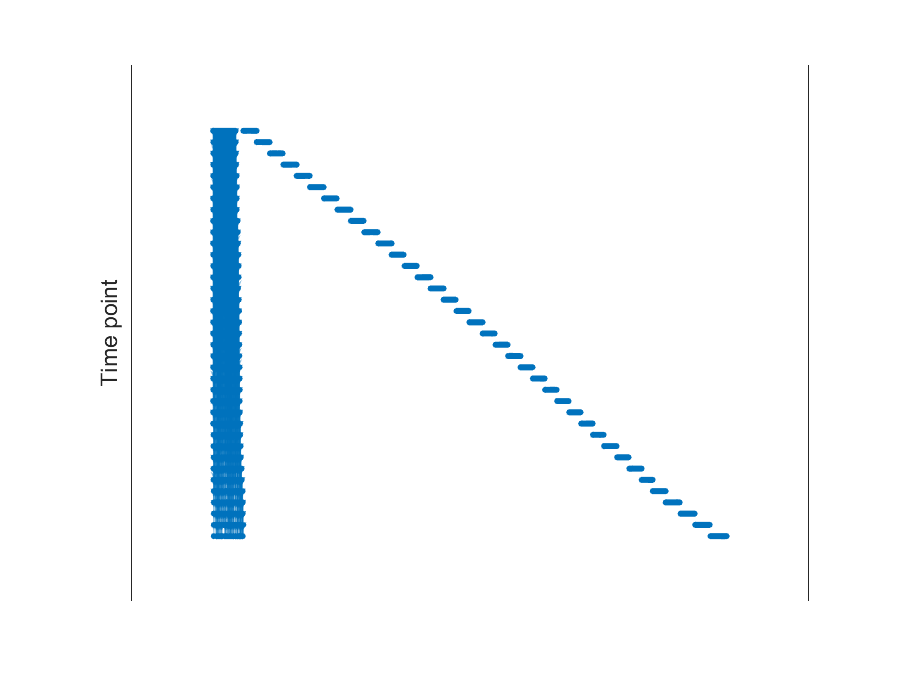
\includegraphics[width=.9\linewidth]{./uncleaned_graph.eps}
\end{center}
cleaning removes:
\begin{enumerate}
\item nodes not connected to any other node
\item nodes not discovered in the first frame
\item nodes linked to fewer than 8 (number of baseline frames) nodes, including itself.
\end{enumerate}
\begin{center}
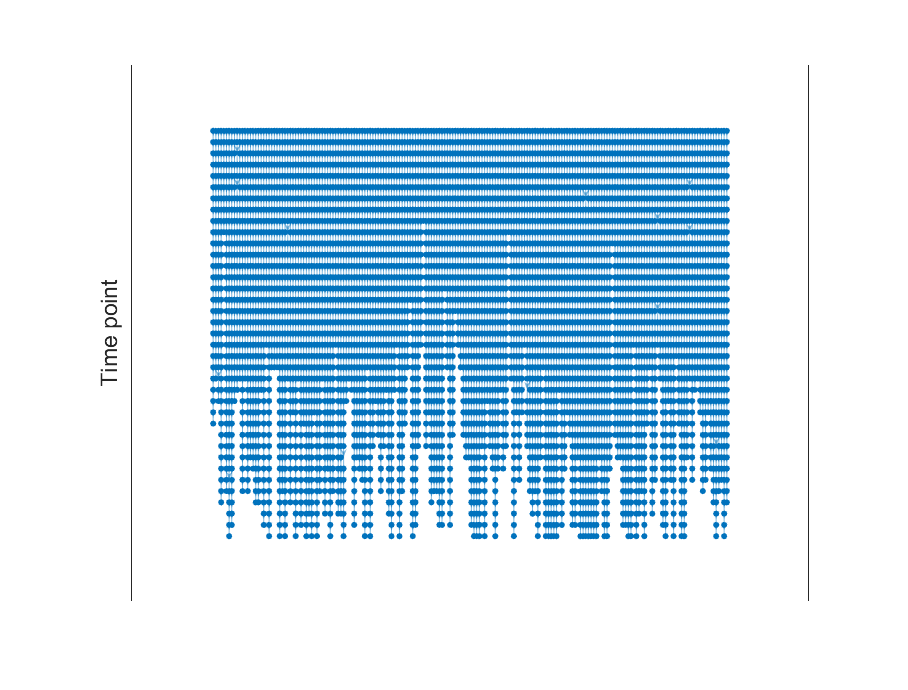
\includegraphics[width=.9\linewidth]{./cleaned_graph.eps}
\end{center}
The fact that the graph edges do not cross link extensively (if at all) suggests the cells do not split/merge much, which is true, suggesting we have good tracking. Let's see the tracks overlayed on the image: 
\begin{center}
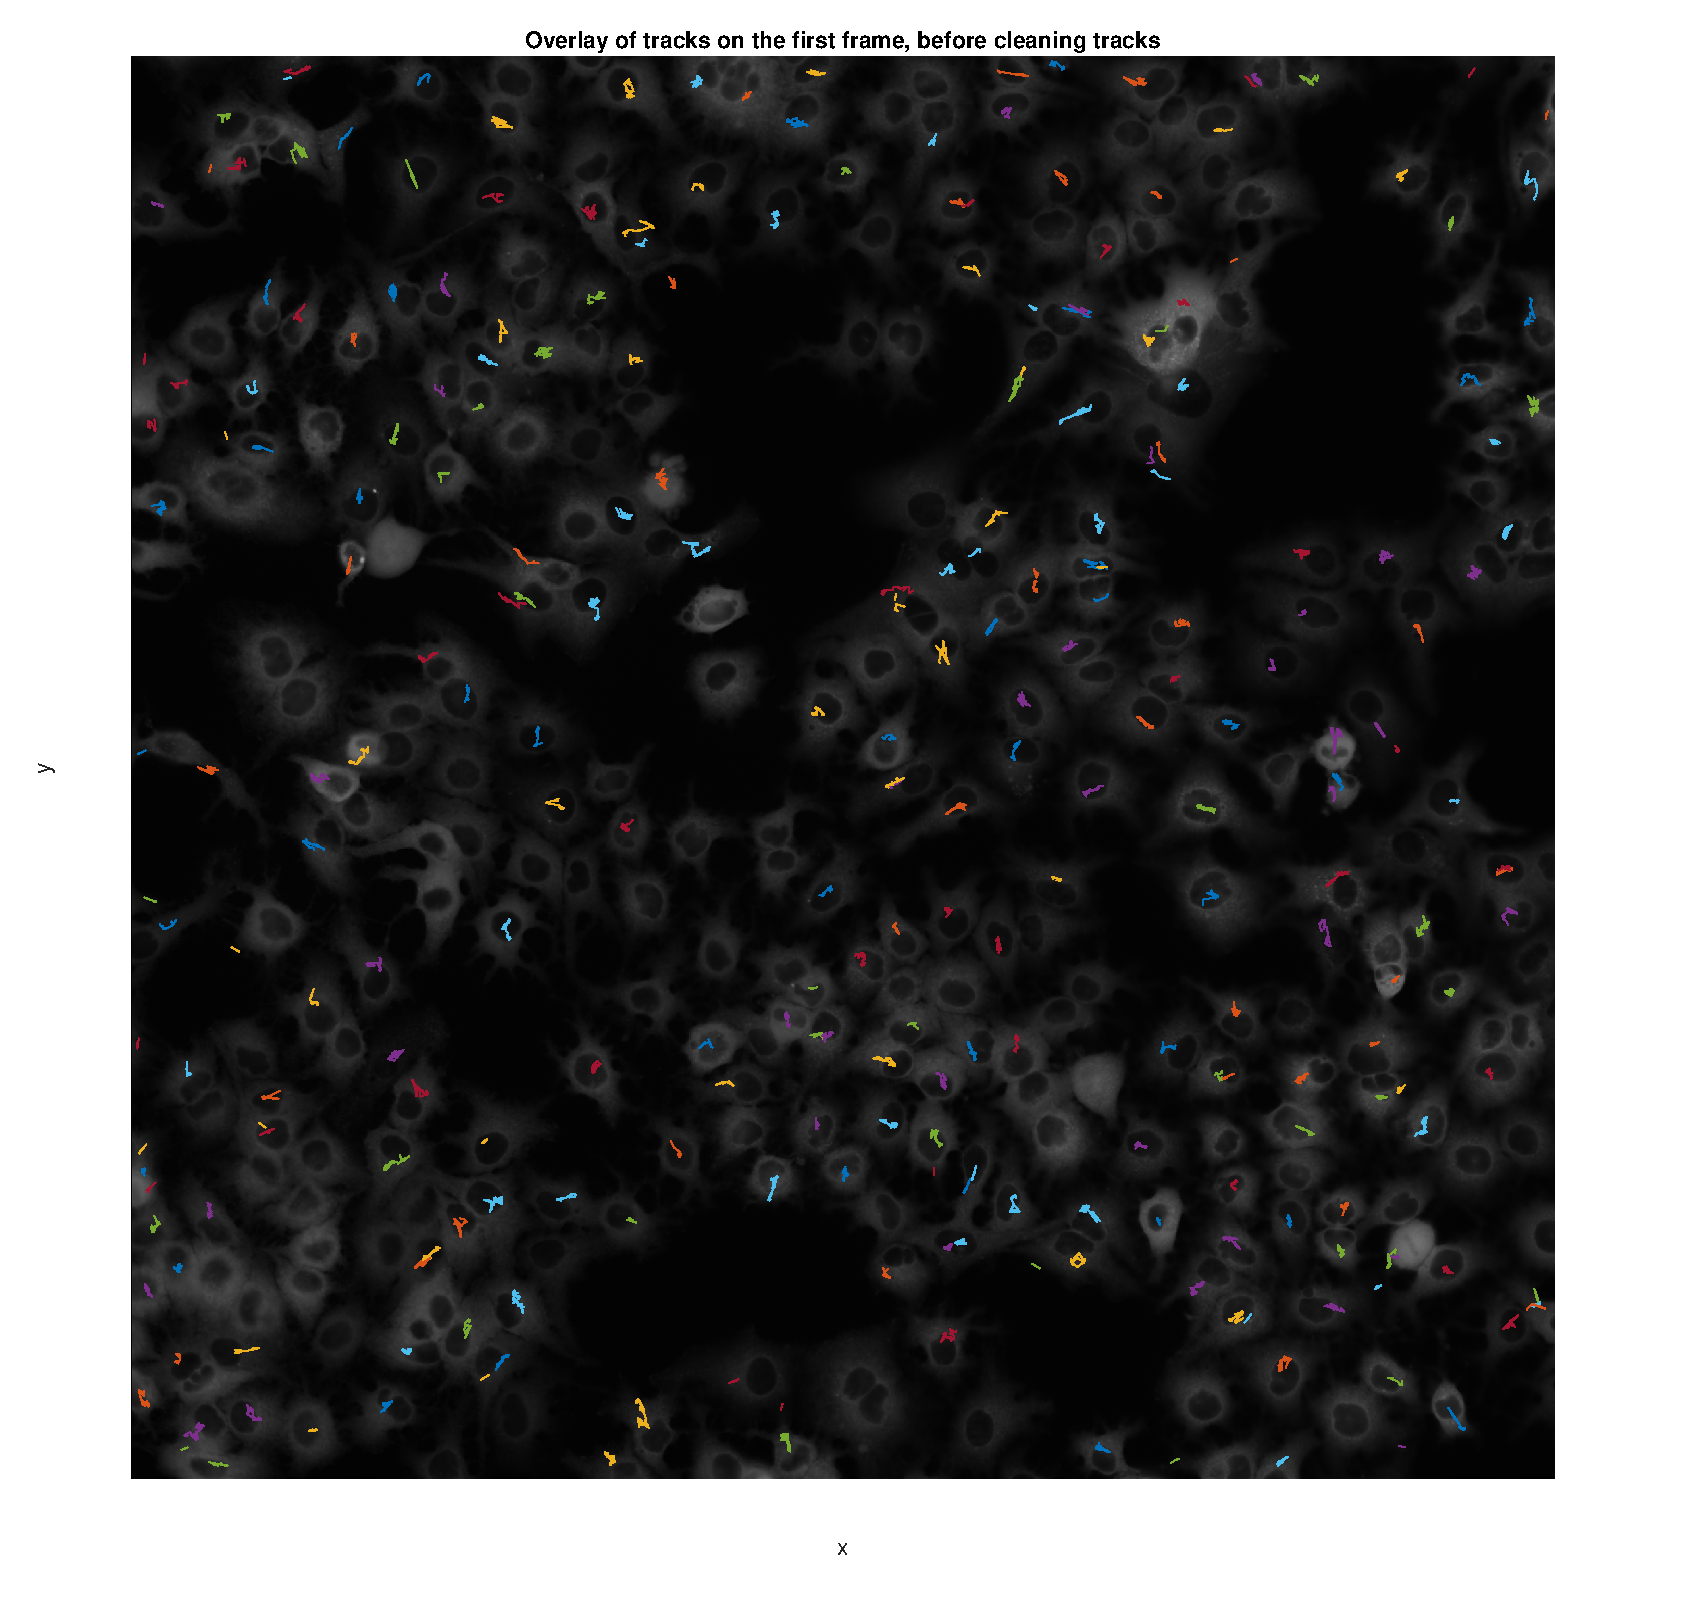
\includegraphics[width=.9\linewidth]{./overlay.eps}
\end{center}
The tracking now indeed works pretty well. However, the intensities are still not very clean:
\begin{center}
\includegraphics[width=.9\linewidth]{./montage-0.png}
\end{center}
\begin{center}
\includegraphics[width=.9\linewidth]{./montage-1.png}
\end{center}
\begin{center}
\includegraphics[width=.9\linewidth]{./montage-2.png}
\end{center}
\begin{center}
\includegraphics[width=.9\linewidth]{./montage-3.png}
\end{center}
\begin{center}
\includegraphics[width=.9\linewidth]{./montage-4.png}
\end{center}
This may be a problem with the mask being inconsistent over the frames. Indeed, the mask seem to persist after the cell has died, catching the ghost images of dead cells: 

\begin{center}
  \includegraphics[width=.9\linewidth]{./37.png}
\end{center}
\begin{center}
  \includegraphics[width=.9\linewidth]{./mask_37.png}
  
\end{center}

This problem can only be fixed with a retrained model. 

\textbf{Note:} the script now does NOT remove nuclei. 
\end{document}